\documentclass[a4paper, 12pt]{article}
\usepackage[utf8]{inputenc}
\usepackage[spanish, provide=*]{babel}
\usepackage{amsmath, amssymb}
\usepackage{graphicx}
\usepackage{hyperref}
\usepackage{listings}
\usepackage{tcolorbox}
\usepackage{xcolor}
\usepackage{fancyhdr}
\usepackage{geometry}

\geometry{left=2.5cm, right=2.5cm, top=3cm, bottom=4.5cm}

% Para las tablas
\usepackage{float}  %Para que no se cambien de lugar
\usepackage{pgfplotstable}
\usepackage{array}
\usepackage{colortbl}
\usepackage{url} % para que el campo note muestre URLs bien

% Estilo
\usepackage{lastpage}

% Definición de colores
\definecolor{cafetitulos}{RGB}{150,75,0}
\definecolor{redv}{RGB}{165, 43, 42}
\definecolor{cafe}{RGB}{130,75,0}
\definecolor{cafet}{RGB}{204, 121, 5}

% Configuración de encabezados y pies de página
\pagestyle{fancy}
\renewcommand{\headrulewidth}{0pt} % Elimina la línea por defecto del encabezado

% Encabezado
\fancyhead[L]{
\includegraphics[height=1.5cm]{logomanual.png}}
\fancyhead[R]{\nouppercase{\leftmark}} % Nombre de la sección

% Pie de página
\renewcommand{\footrulewidth}{0.5pt} % Línea separadora
\renewcommand{\footrule}{\hbox to\headwidth{\color{cafe}\leaders\hrule height \footrulewidth\hfill}}
\fancyfoot[L]{Manual de usuario ChibchaWeb: Empleados - 2025}
\fancyfoot[C]{}
\fancyfoot[R]{Página \thepage} % Número de página a la derecha

% Ajustar altura del encabezado y espacio para el pie
\setlength{\headheight}{52pt} % Altura del encabezado (ajusta según el logo)
\setlength{\footskip}{40pt} % Espacio entre el texto y el pie (evita solapamiento)

% Titulos
\usepackage{titlesec} % Para personalizar section/subsection
\titleformat{\section}
  {\normalfont\Large\bfseries}{\thesection}{1em}{\color{cafetitulos}} % Section en café
\titleformat{\subsection}
  {\normalfont\bfseries}{\thesubsection}{1em}{\color{cafe}}
\titleformat{\subsubsection}{\normalfont\bfseries}{\thesubsubsection}{1em}{\color{cafetitulos}}

% Configuración para código fuente
\lstset{
    language=Java, % puedes cambiar a Python, SQL, etc.
    basicstyle=\ttfamily\small,
    backgroundcolor=\color{gray!10},
    frame=single,
    breaklines=true,
    keywordstyle=\color{cafetitulos},
    commentstyle=\color{gray},
    stringstyle=\color{redv}
}


\title{

\includegraphics[width=5cm]{logo.png}\\

{\Large CHIBCHAWEB HOSTING PLATFORM}\\
{\Large APLICACIÓN PARA UNA COMPAÑÍA DE HOSPEDAJE DE PÁGINAS WEB}\\[0.5em]

\textbf{MANUAL USUARIO EMPLEADOS}\\[0.5em]
}
\author{
\textbf{Grupo A}\\[0.5em]
Ingenieros:\\
Andrés José Acevedo Ardila\\
Brayan Steven Sánchez Casilima\\
Christian Camilo Lancheros Sánchez\\
Juan Esteban Ordoñez Sandoval\\
Karen Tatiana Bravo Rodríguez\\
Luis Felipe Mayorga Tibaquicha\\\\\\
Universidad Distrital Francisco José de Caldas\\
Facultad de Ingeniería\\
Ingeniería de sistemas\\
}
\date{Bogotá D.C., Agosto 2025}


% Inicio Documento
\begin{document}
\maketitle
\newpage
\begin{titlepage}
\newgeometry{left=2cm, right=0cm, top=2cm, bottom=2cm} % sin margen derecho
\thispagestyle{empty}

\begin{tikzpicture}[remember picture, overlay]
    \node[anchor=north east, inner sep=0pt, xshift=12cm] at (current page.north east) {
        
\includegraphics[height=\paperheight]{registro-imagen.png}
    };
\end{tikzpicture}

\vfill
{
\includegraphics[width=0.6\textwidth]{logomanual.png}\par}
\vfill
{\Huge Grupo A\par}
{\Huge Manual Técnico ChibchaWeb\par}
{\Large 2025\par}
\vfill


\end{titlepage}


\newpage
\tableofcontents

\newpage
\listoffigures

\newpage
\section{Introducción}
Este manual proporciona la información necesaria para la instalación, configuración, operación y mantenimiento del sistema ChibchaWeb, una plataforma web orientada al servicio de hospedaje de sitios web. El sistema permite la gestión de cuentas de clientes, distribuidores y empleados, la adquisición de dominios, facturación automática, administración de tickets de soporte, y más. Esta guía está dirigida a desarrolladores, administradores del sistema y personal técnico encargado del mantenimiento de la solución. \\

El manual técnico documenta el desarrollo e instalación de un sistema web que automatiza las operaciones clave de ChibchaWeb, incluyendo: 

\begin{enumerate}
    \item {Registro y gestión de cuentas de clientes, empleados y distribuidores.}
    \item {Validación de información sensible como direcciones y tarjetas de crédito.}
    \item {Procesamiento de pagos mediante tarjetas aceptadas (VISA, MASTERCARD, DINERS).}
    \item {Administración de dominios y envío de solicitudes a registradores externos.}
    \item {Registro y gestión de tickets de soporte técnico.}
    \item {Cálculo de comisiones para distribuidores y generación de archivos de transferencia. }
\end{enumerate}

El objetivo de esta documentación es proporcionar una guía técnica completa que facilite la instalación, configuración, uso, mantenimiento y actualización del sistema para desarrolladores, administradores del sistema y personal técnico de soporte. 

\newpage
\section{Roles y funciones}
\subsection{Cliente}
Persona natural o jurídica que contrata los servicios de hospedaje web ofrecidos por ChibchaWeb.
Puede elegir entre diferentes paquetes (Chibcha-Platino, Chibcha-Plata, Chibcha-Oro) y planes de pago (mensual, trimestral, semestral o anual).
Sus responsabilidades incluyen:

\begin{itemize}
\item Proporcionar información personal y de contacto válida.

\item Seleccionar y mantener actualizado su método de pago.

\item Solicitar registro o transferencia de dominios si así lo requiere.

\item Reportar incidencias o solicitudes de soporte técnico a través del sistema.
\end{itemize}

\subsection{Distribuidor}

Entidad o persona autorizada por ChibchaWeb para comercializar y revender sus servicios de hospedaje web a terceros.
Está clasificado en dos categorías según el número de dominios administrados:

\begin{itemize}
    \item BÁSICO: Hasta 100 dominios (10% de comisión).
    \item PREMIUM: Más de 100 dominios (15% de comisión).
\end{itemize}

Sus responsabilidades incluyen:

\begin{itemize}
    \item Gestionar sus propios clientes y procesar los pagos correspondientes.
    \item Administrar y mantener actualizada su cartera de dominios.
    \item Tramitar solicitudes de registro o transferencia de dominios a través de ChibchaWeb.
    \item Cumplir con las políticas y acuerdos comerciales establecidos.
\end{itemize}


\newpage
\section{Acceso al sistema}
\subsection{Requisitos}
Debe cumplir con una serie de requisitos técnicos mínimos para poder hacer uso de este, como son:

\begin{itemize}
	\item Conexión a internet

\item Sistema operativo:
    \begin{itemize}
        \item Windows 10/11
        \item Linux
    \end{itemize}

\item Navegador con versión minima:
    \begin{itemize}
    \item Google Chrome: 100+
    \item Mozilla: 100+
    \item Microsoft Edge: 100+
    \item Safari (macOS): 15+
    \item Opera: 85+
    \item Safari (iOS): 15+
    \item Chrome/Edge Android: Última versión
    \end{itemize}
\end{itemize}

En cuando cumpla con los requisitos anteriormente mencionados, puede continuar con el proceso de registro e inicio de sesión, de la siguiente manera:

\subsection{Acceso al sistema}

Para el acceso al sistema se cuenta con la url de acceso siguiente:

\url{ https://www.chibchaweb.site/}\\

Se encontrará en la pestaña de inicio del sitio web, donde podrá explorar los dominios, sin necesidad de registrarse.

\begin{figure}[H]
    \centering
	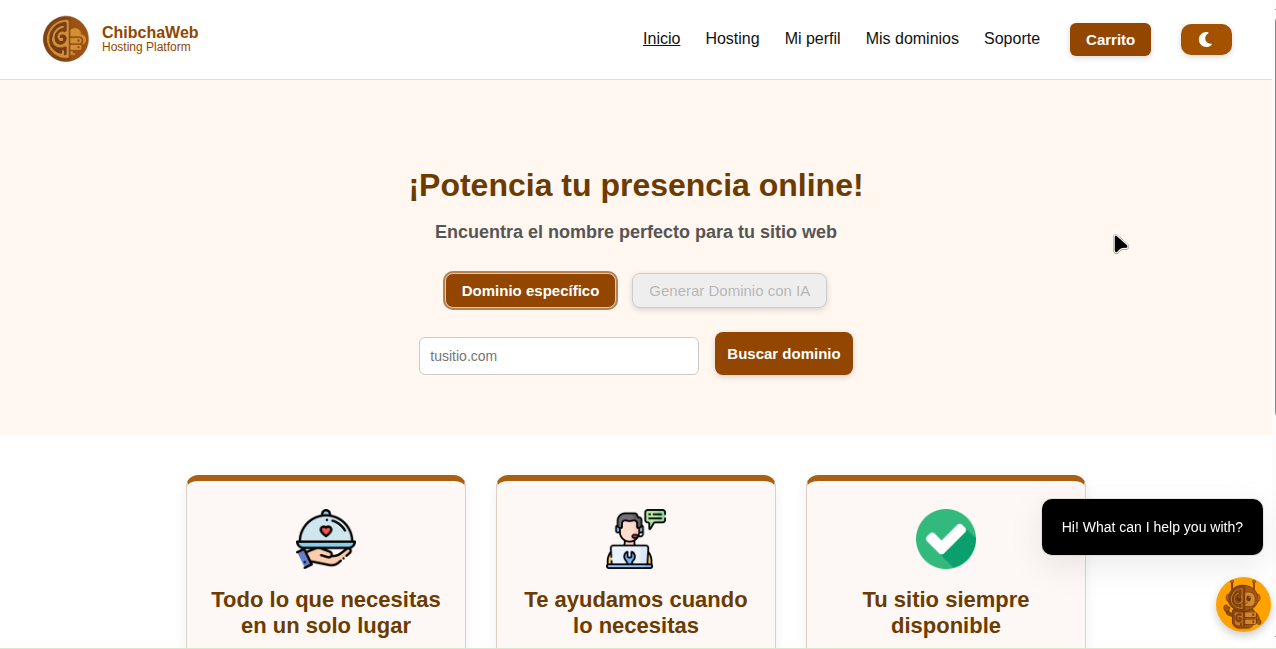
\includegraphics[width=0.8\linewidth]{acceso/inicio.png}
	\caption{Página principal.}
	\label{fig:inicio}
\end{figure}

\subsection{Registro de usuario }
El registro de usuario Solo se puede realizar como empleado, no como Administrador, para registrarse cómo empleado, se debe llenar el siguiente formulario:

\begin{figure}[H]
    \centering
    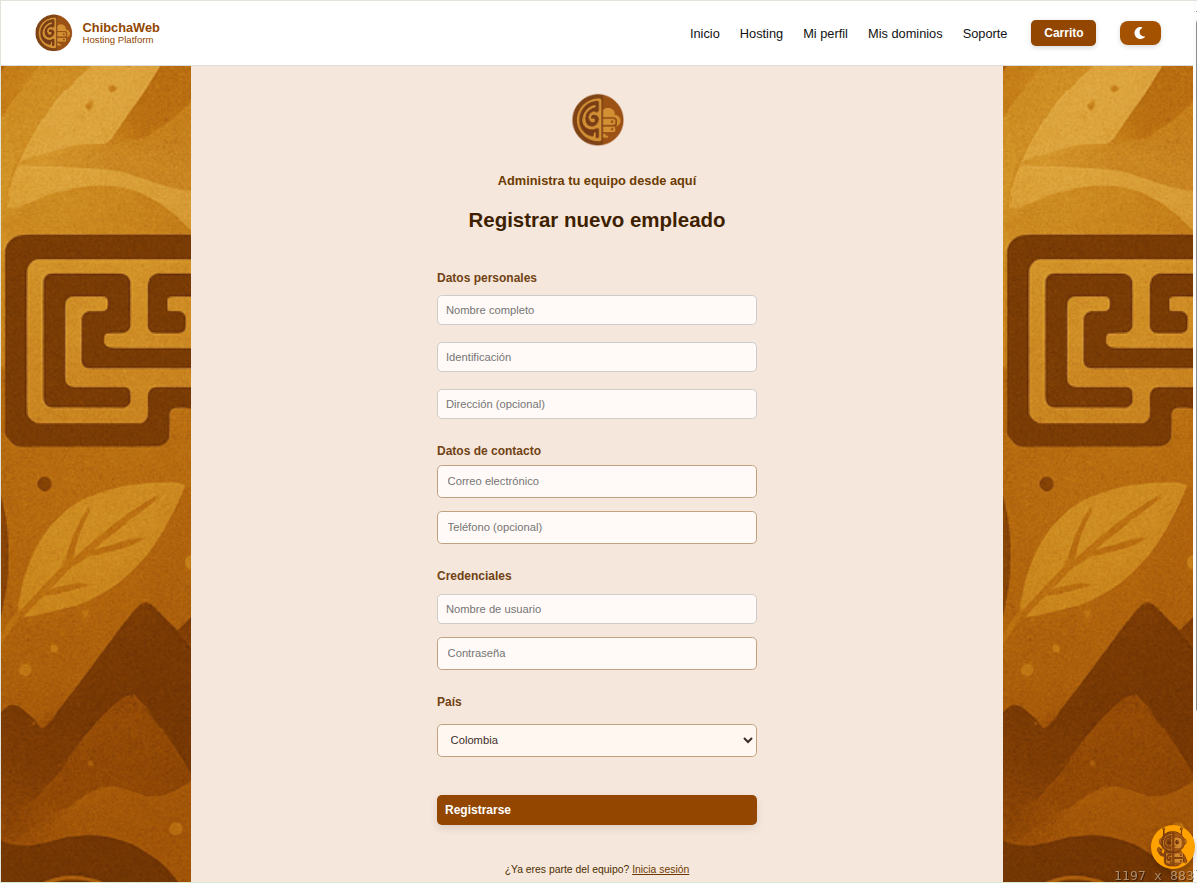
\includegraphics[width=0.8\linewidth]{acceso/registro-empleado.png}
    \caption{Registro empleado.}
    \label{fig:registro-empleado}
\end{figure}

Posteriormente, debe esperar a ser notificado de que su cuenta ha sido validada por un administrador.

Luego de esto será redirigido al inicio de sesión.

\subsection{Inicio de sesión}
Para el inicio de sesión, deberá ingresar su identificador de usuario, y su contraseña en los espacios que se ven en la Figura \ref{fig:login} En caso de no contar con una cuenta, revise el punto anterior.

\begin{enumerate}
	\item Dar click en el botón de “Mi perfil” que se encuentra en la barra de navegación.
	\begin{figure}[H]
		
\includegraphics[width=\columnwidth]{acceso/navbar-perfil.png}
		\caption{Barra de navegación.}
		\label{fig:navbar-perfil}
	\end{figure}
    \item Deberá ingresar sus credenciales, y dar click en “Entrar”.
    \begin{figure}[H]
        \centering
  		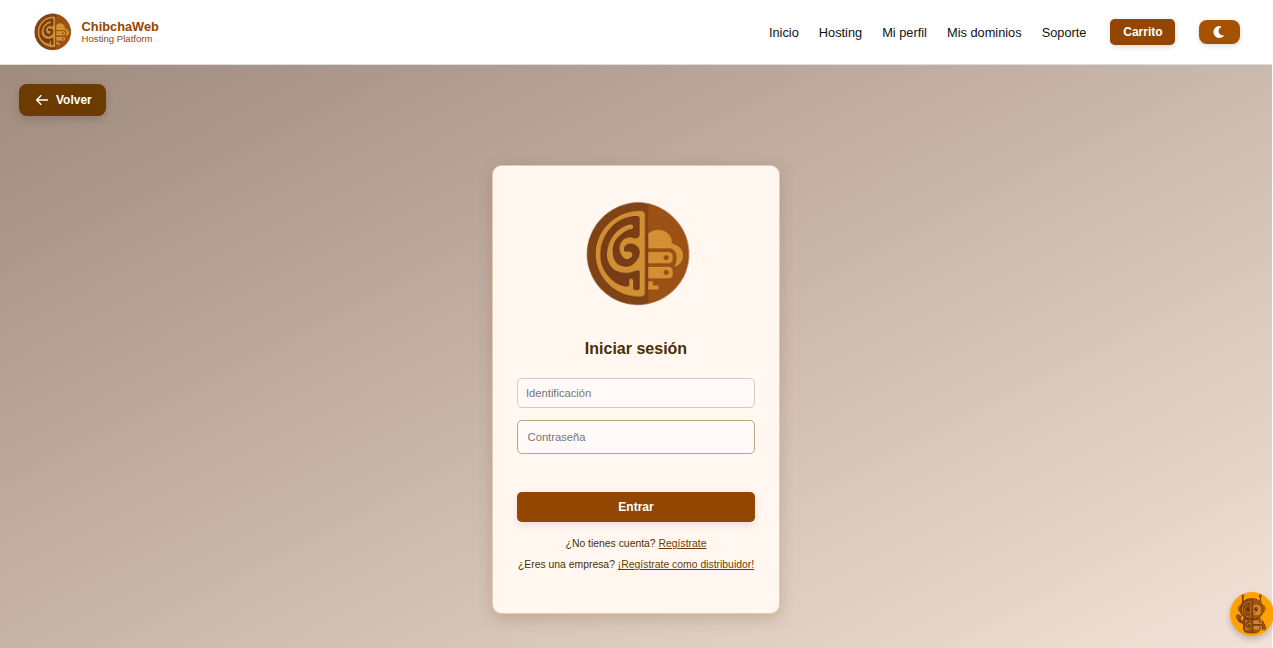
\includegraphics[width=\columnwidth]{acceso/login.png}
  		\caption{Login.}
  		\label{fig:login}
   	\end{figure}
\end{enumerate}

Luego de clic en entrar, donde deberá ver una interfaz similar a la siguiente

\begin{figure}[H]
    \centering
    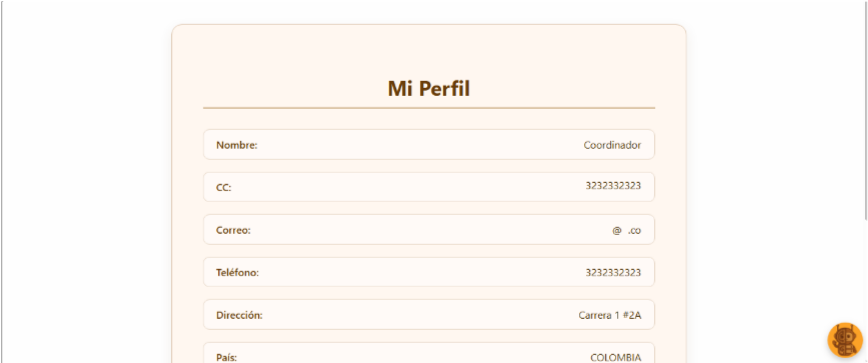
\includegraphics[width=\columnwidth]{acceso/perfil.png}
    \caption{Datos de mi perfil.}
    \label{fig:placeholder}
\end{figure}


\newpage
\section{Guía paso a paso por módulo}
\subsection{Técnico}
Para acceder, deberá ingresar con un perfil de tipo Técnico, donde luego de iniciar sesión, observará el siguiente menú:

\subsubsection*{Visualiza y gestionar tickets}

\begin{enumerate}
	\item Para acceder, deberá ingresar con un perfil de tipo Técnico, donde luego de iniciar sesión, observará el siguiente menú:
   	\begin{figure}[H]
    \centering
    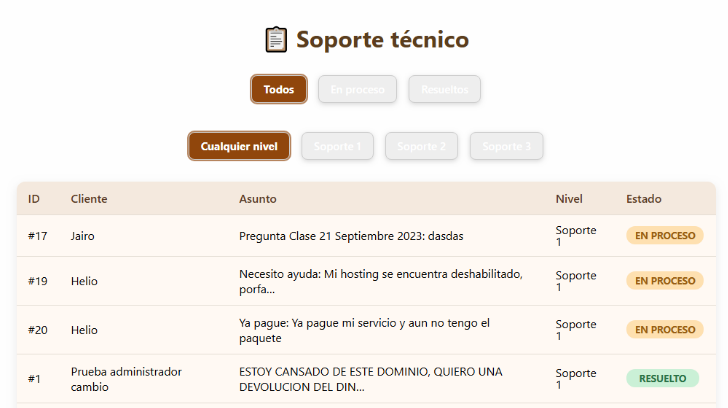
\includegraphics[width=0.75\linewidth]{guiamodulo/tecnico-menu.png}
    \caption{Feed general técnico.}
    \label{fig:tecnico-menu}
    \end{figure}

    \item Donde podrá Visualizar los tickets y editar su estado
    \begin{figure}[H]
    \centering
    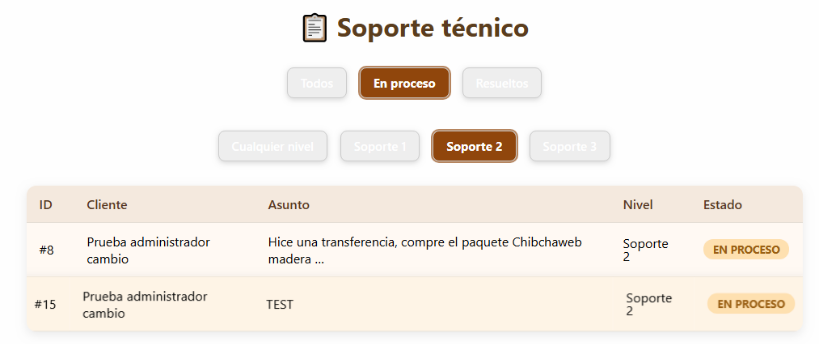
\includegraphics[width=0.75\linewidth]{guiamodulo/tecnico-proceso.png}
    \caption{Feed "En proceso" técnico.}
    \label{fig:tecnico-proceso}
    \end{figure}
\end{enumerate}

\subsection{Coordinador}
Para acceder, deberá ingresar con un perfil de tipo Coordinador sin importar el nivel, donde luego de iniciar sesión, observará el siguiente menú:

\begin{figure}[H]
    \centering
    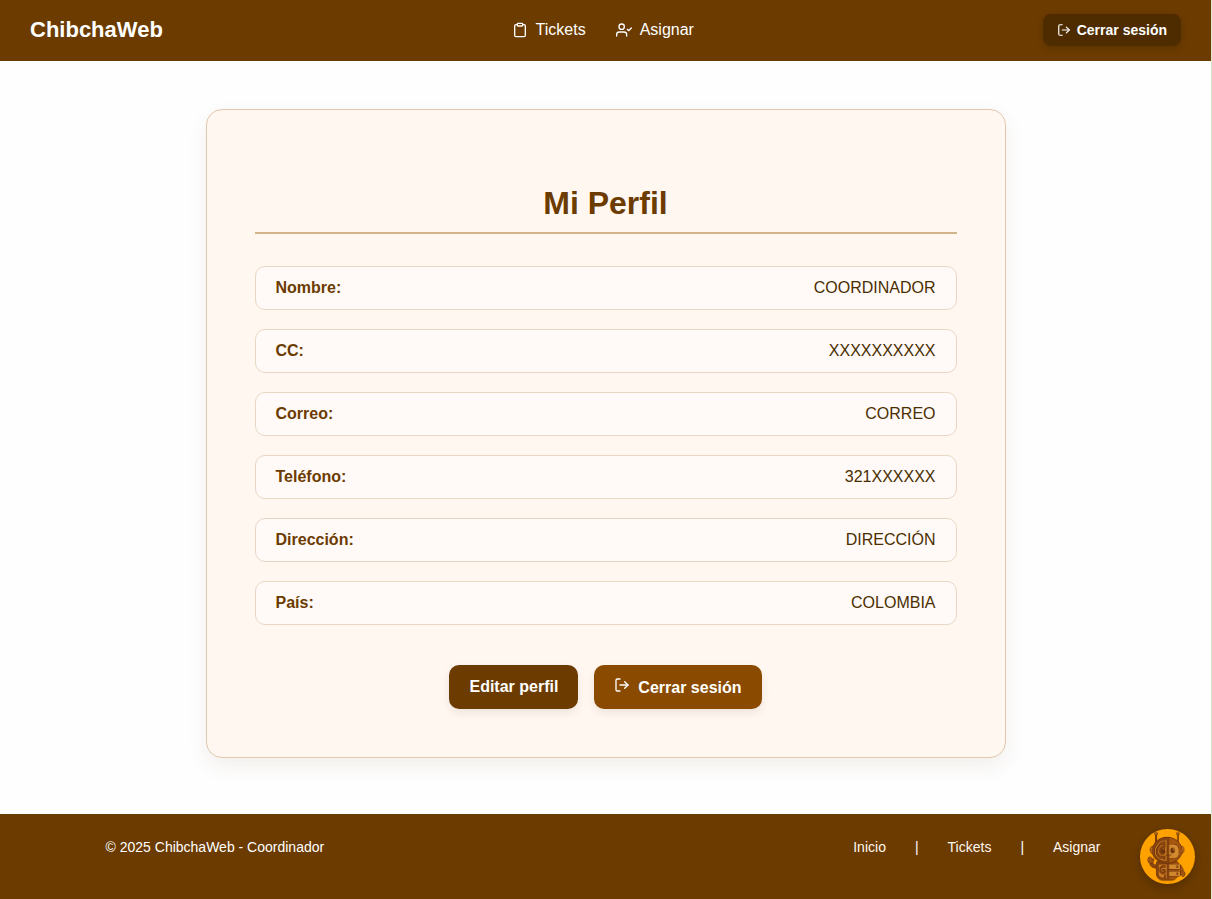
\includegraphics[width=0.75\linewidth]{guiamodulo/perfil-coordinador.png}
    \caption{Perfil Coordinador.}
    \label{fig:perfil-coordinador}
\end{figure}

Con este perfil, podrá realizar las siguientes acciones:

\begin{enumerate}
    \item Gestión de Tickets.
    \item Asignación de tickets.
\end{enumerate}

A continuación se describe como realizar cada una de las acciones:

\subsubsection{Gestión de tickets }
\begin{enumerate}
    \item Dar click en la pestaña "Tickets".
        \begin{figure}[H]
        \centering
        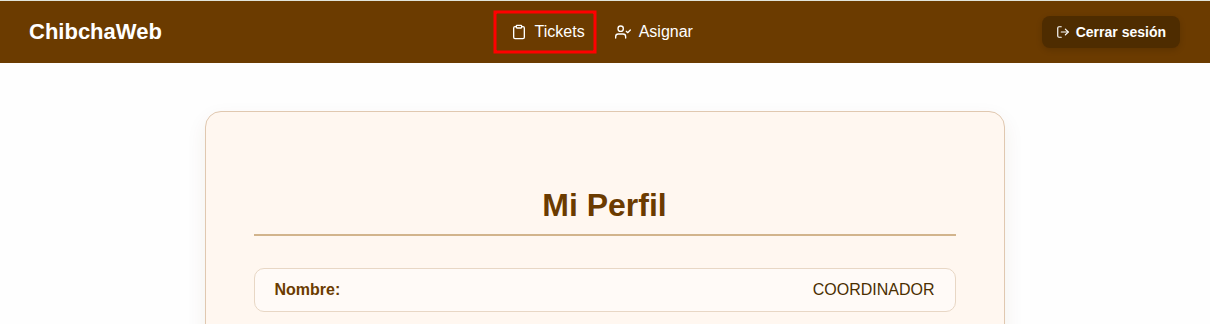
\includegraphics[width=0.8\linewidth]{guiamodulo/navbar-coo-tickect.png}
        \caption{Barra de navegación coordinador, Tickets.}
        \label{fig:navbar-coo-tickect}
        \end{figure}
    \item Allí podrá observar 3 categorias de tickets según el estado en el que se encuentren: Sin asignar, En proceso, Terminado.
        \begin{figure}[H]
            \centering
            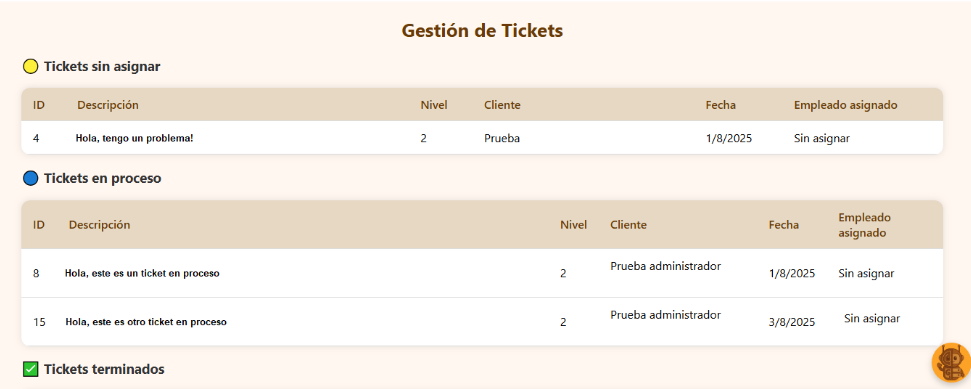
\includegraphics[width=0.8\linewidth]{guiamodulo/coordinador-tickets.png}
            \caption{Feed de tickets del coordinador.}
            \label{fig:coordinador-tickets}
        \end{figure}
\end{enumerate}

\subsubsection{Asignación de tickets }
\begin{enumerate}
    \item Para ello se debe ingresar a “Asignar”, de la siguiente manera:
        \begin{figure}[H]
        \centering
        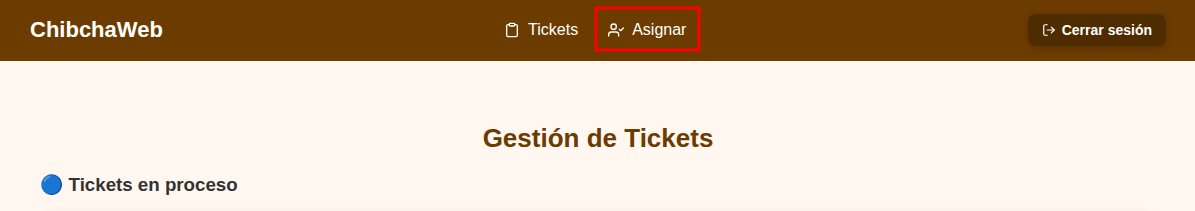
\includegraphics[width=0.8\linewidth]{guiamodulo/navbar-coo-asignar.png}
        \caption{Barra de navegación coordinador, Asignar.}
        \label{fig:navbar-coo-asignar}
        \end{figure}
    \item Donde se encontrarán los tickets disponibles, y podrá asignarlos a un empleado de soporte, o escalarlo.
        \begin{figure}[H]
            \centering
            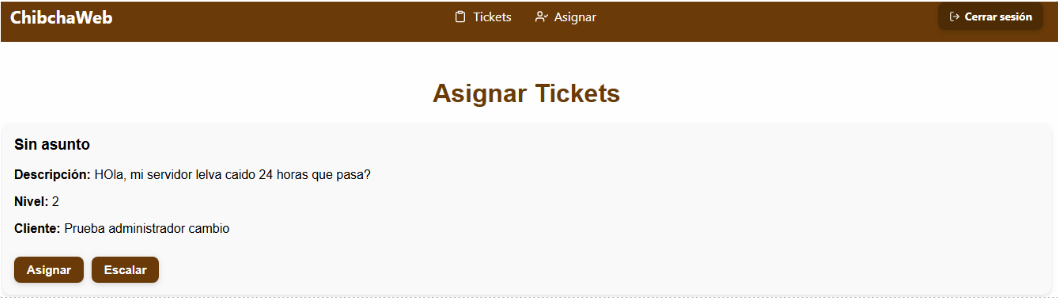
\includegraphics[width=0.8\linewidth]{guiamodulo/coordinador-asignar.png}
            \caption{Enter Caption}
            \label{fig:placeholder}
        \end{figure}
\end{enumerate}


\subsection{Administrador}
Para acceder, deberá ingresar con un perfil de tipo Administrador, donde luego de iniciar sesión, observará el siguiente menú:
\begin{figure}[H]
    \centering
    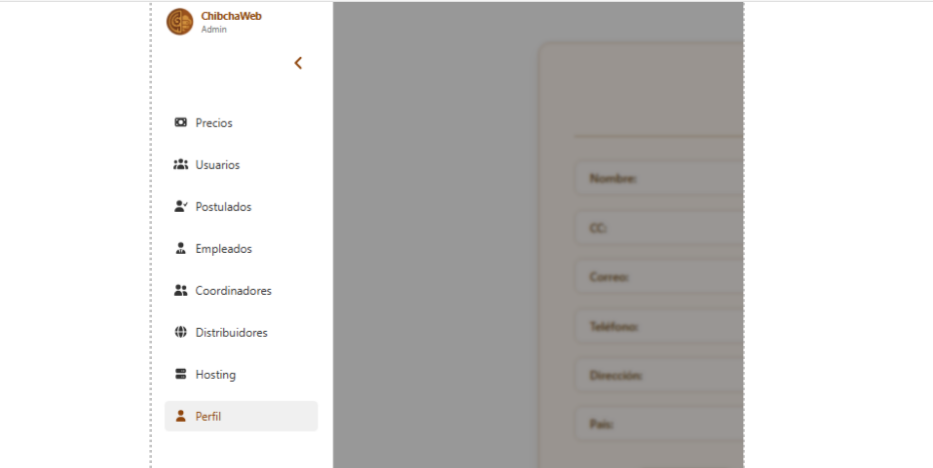
\includegraphics[width=1\linewidth]{guiamodulo/menu-admin.png}
    \caption{Menú Administrador}
    \label{fig:menu-admin}
\end{figure}

Con este perfil, podrá realizar las siguientes acciones:

\begin{itemize}
    \item{Modificar Precios de dominios}
    \item{Gestionar Usuarios}
    \item{Gestionar Empleados}
    \item{Gestionar Distribuidores}
    \item{Gestionar planes de Hosting}
    \item{Gestionar perfil}
\end{itemize}

A continuación, se describen como realizar cada una de ellas

\subsubsection{Modificar Precios de dominios}
\begin{enumerate}
    \item Para realizar esta acción, se debe dar clic en “Precios” del menú del administrador visto en la figura \ref{fig:menu-admin}.
    \begin{figure}[H]
        \centering
        
\includegraphics[width=0.3\linewidth]{guiamodulo/menu-admin-precios.png}
        \caption{Menú Admin, botón Precios}
        \label{fig:menu-admin-precios}
    \end{figure}

    \item Seleccionar la extensión a la que se desea modificar el precio, y editarlo
    \begin{figure}[H]
        \centering
        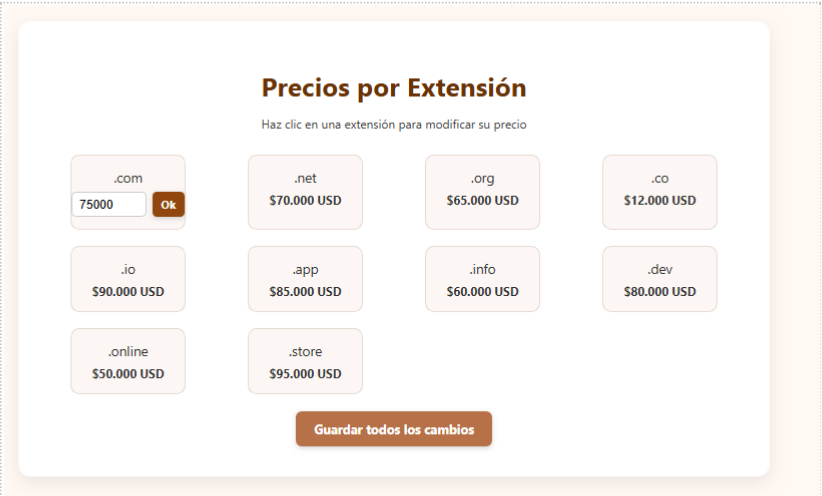
\includegraphics[width=0.7\linewidth]{guiamodulo/mod-precios.png}
        \caption{Modificar precios de por extensión.}
        \label{fig:mod-precios}
    \end{figure}

     \item Seleccionar el botón “Guardar todos los cambios”
    \begin{figure}[H]
        \centering
        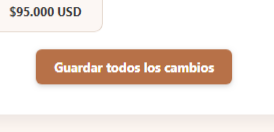
\includegraphics[width=0.4\linewidth]{guiamodulo/mod-precios-guardar.png}
        \caption{Modificar precios de por extensión, guardar.}
        \label{fig:mod-precios-guardar}
    \end{figure}

    \item  Si todo se realizó de la forma correcta, se mostrará el siguiente aviso:
    \begin{figure}[H]
        \centering
        
\includegraphics[width=0.75\linewidth]{guiamodulo/mod-precios-aviso.png}
        \caption{Modificar precios de por extensión, notificación.}
        \label{fig:mod-precios-aviso}
    \end{figure}
\end{enumerate}


\subsubsection{Gestionar Usuarios}
\begin{enumerate}
    \item Para realizar esta acción, se debe dar clic en el botón “Usuarios” del menú del administrador visto en la figura \ref{fig:menu-admin}.
visto en la figura
        \begin{figure}[H]
            \centering
            
\includegraphics[width=0.3\linewidth]{guiamodulo/menu-admin-usuarios.png}
            \caption{Mené Admin, botón Usuarios}
            \label{fig:menu-admin-usuarios}
        \end{figure}

    \item Donde podrá buscar y seleccionar los clientes registrados
    \begin{figure}[H]
        \centering
        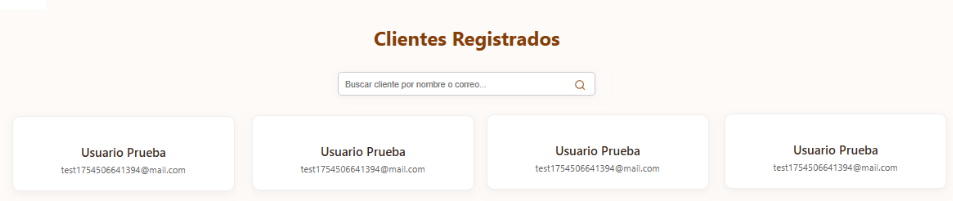
\includegraphics[width=0.8\linewidth]{guiamodulo/admin-usuarios-registrados.png}
        \caption{Admin, usuarios registrados.}
        \label{fig:admin-usuarios-registrados}
    \end{figure}

    \item Accediendo al detalle del cliente, y decidir si editar su información, o eliminar la cuenta
    \begin{figure}[H]
        \centering
        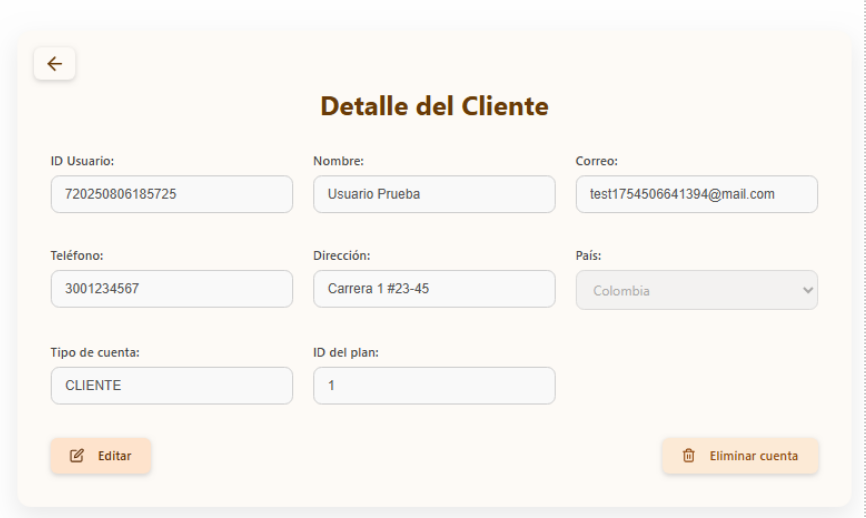
\includegraphics[width=0.75\linewidth]{guiamodulo/admin-usuario-detalle.png}
        \caption{Admin, detalle usuario.}
        \label{fig:admin-usuario-detalle}
    \end{figure}
\end{enumerate}

\subsubsection{Gestionar Postulados}
\begin{enumerate}
    \item Para realizar esta acción, se debe dar clic en “Postulados”
    \begin{figure}[H]
        \centering
        
\includegraphics[width=0.3\linewidth]{guiamodulo/menu-admin-postulados.png}
        \caption{Menú Admin, postulados.}
        \label{fig:menu-admin-postulados}
    \end{figure}

    \item Seleccione el empleado que desea aceptar
    \begin{figure}[H]
        \centering
        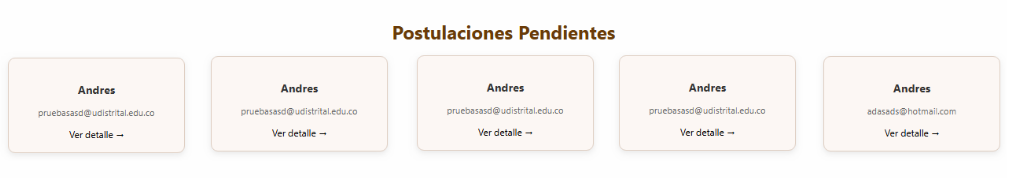
\includegraphics[width=0.8\linewidth]{guiamodulo/admin-postulados.png}
        \caption{Postulados.}
        \label{fig:admin-postulados}
    \end{figure}

    \item Seleccione el nivel de soporte y clic en el boton “Asignar nivel”
    \begin{figure}[H]
        \centering
        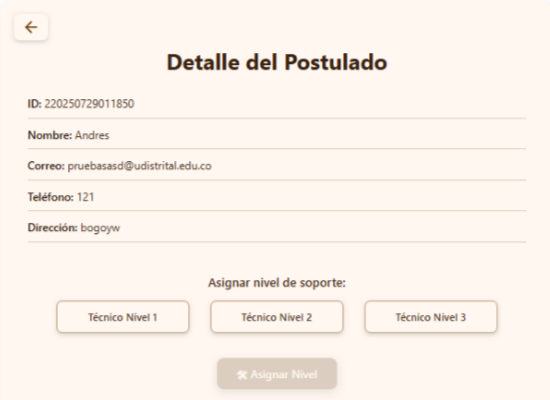
\includegraphics[width=0.6\linewidth]{guiamodulo/admin-postulados-detalle.png}
        \caption{Detalle postulado.}
        \label{fig:admin-postulados-detalle}
    \end{figure}
\end{enumerate}

\subsubsection{Gestionar Empleados}

\begin{enumerate}
\item Para realizar esta acción, se debe dar clic en “Empleados”

\begin{figure}[H]
    \centering
    
\includegraphics[width=0.3\linewidth]{guiamodulo/menu-admin-empleados.png}
    \caption{Menú Admin, empleados.}
    \label{fig:menu-admin-empleados}
\end{figure}

\item  Seleccionar el técnico deseado y dar clic en “Reasignar”

\begin{figure}[H]
    \centering
    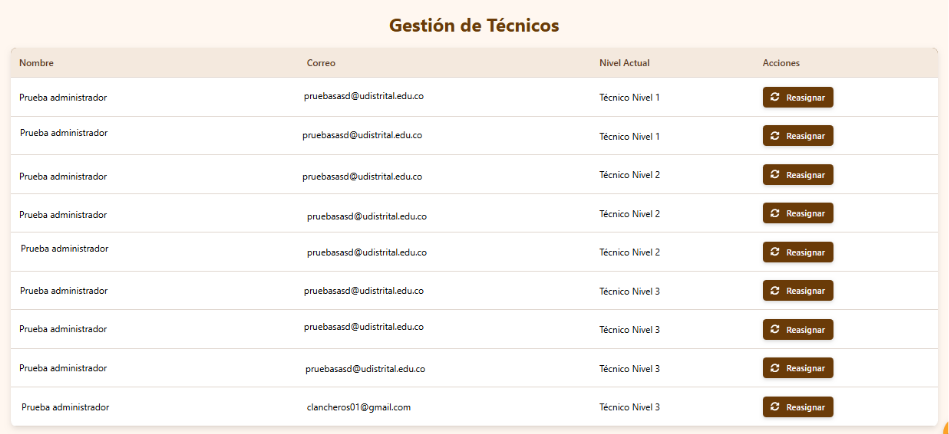
\includegraphics[width=0.7\linewidth]{guiamodulo/gestion-tecnicos.png}
    \caption{Gestión técnicos.}
    \label{fig:gestion-tecnicos.png}
\end{figure}

\item Seleccionar el nuevo nivel de técnico a asignar, y dar clic en “Guardar”

\begin{figure}[H]
    \centering
    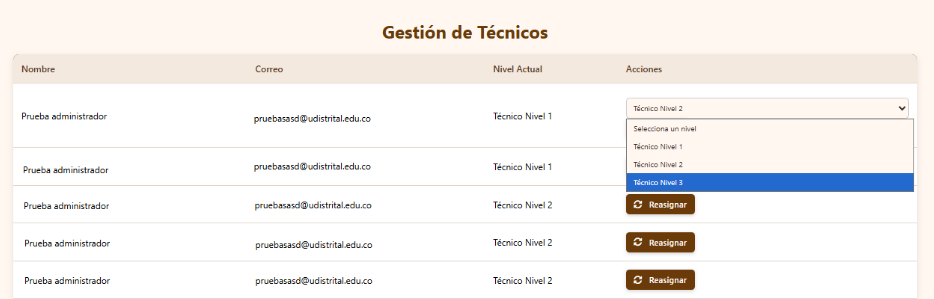
\includegraphics[width=0.7\linewidth]{guiamodulo/gestion-tecnicos-menu.png}
    \caption{Gestión técnicos, selección niveles.}
    \label{fig:gestion-tecnicos-menu.png}
\end{figure}

\item Si todo salió bien, se observará el anuncio de actualización, de la siguiente manera

\begin{figure}[H]
    \centering
    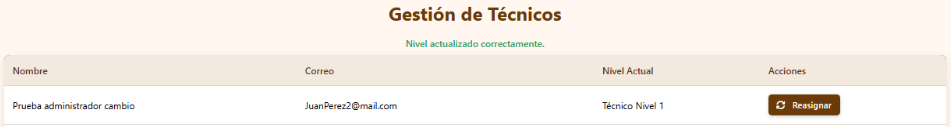
\includegraphics[width=0.7\linewidth]{guiamodulo/gestion-tecnicos-aviso.png}
    \caption{Gestión técnicos, notificación.}
    \label{fig:gestion-tecnicos-aviso.png}
\end{figure}

\end{enumerate}

\subsubsection{Gestionar Coordinadores}

\begin{enumerate}
\item Para realizar esta acción, se debe dar clic en “Coordinadores”

\begin{figure}[H]
    \centering
    
\includegraphics[width=0.3\linewidth]{guiamodulo/menu-admin-coordinadores.png}
    \caption{Menú Admin, coordinadores.}
    \label{fig:menu-admin-coordinadores}
\end{figure}

\item Igual que el punto anterior, se debe seleccionar el nuevo nivel y guardar

\begin{figure}[H]
    \centering
    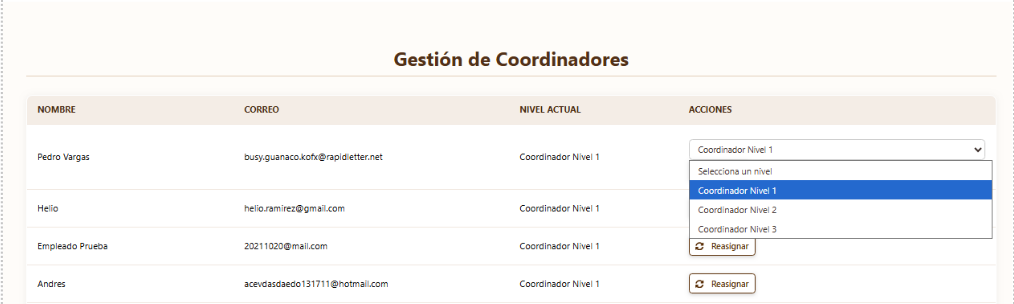
\includegraphics[width=0.7\linewidth]{guiamodulo/gestion-coordinadores.png}
    \caption{Gestión coordinadores.}
    \label{fig:gestion-coordinadores.png}
\end{figure}

\item Si todo salió bien, se observará el anuncio de actualización, de la siguiente manera

\begin{figure}[H]
    \centering
    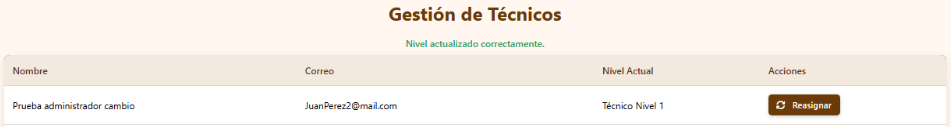
\includegraphics[width=0.7\linewidth]{guiamodulo/gestion-tecnicos-aviso.png}
    \caption{Gestión coordinadores, notificación.}
    \label{fig:gestion-coordinadores-aviso.png}
\end{figure}

\end{enumerate}


\subsubsection{Gestionar Distribuidores}

 \begin{enumerate}
 \item Para realizar esta acción, se debe dar clic en “Distribuidores”
 \begin{figure}[H]
     \centering
     
\includegraphics[width=0.3\linewidth]{guiamodulo/menu-admin-distribuidores.png}
     \caption{Menú Admin, distribuidores.}
     \label{fig:menu-admin-distribuidores}
 \end{figure}

 \item Seleccione el distribuidor a consultar
 \begin{figure}[H]
     \centering
     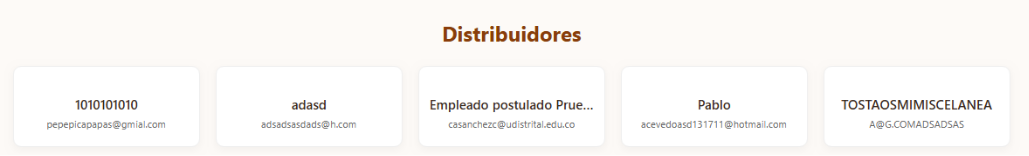
\includegraphics[width=0.7\linewidth]{guiamodulo/gestion-distribuidores.png}
     \caption{Gestión distribuidores.}
     \label{fig:gestion-distribuidores.png}
 \end{figure}

 \item Edite la información del distribuidor
 \begin{figure}[H]
     \centering
     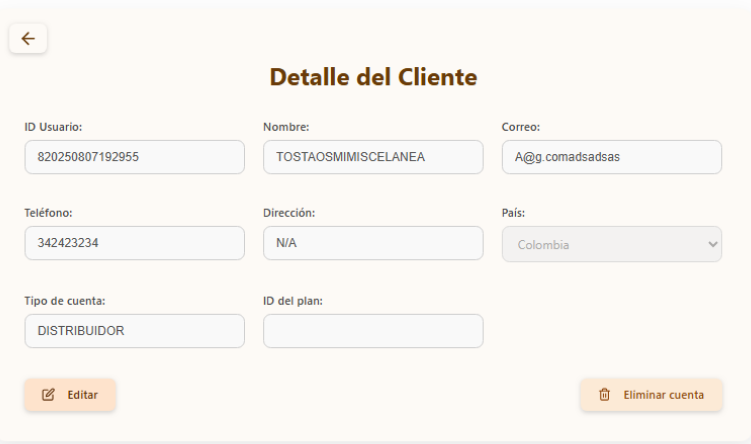
\includegraphics[width=0.7\linewidth]{guiamodulo/gestion-distribuidores-detalle.png}
     \caption{Gestión distribuidores detalle.}
     \label{fig:gestion-distribuidores-detalle.png}
 \end{figure}

 \end{enumerate}


\subsubsection{Gestionar planes de Hosting}

\subsubsection*{Editar paquete de Hosting}

\begin{enumerate}
    \item Para realizar esta acción, se debe dar clic en “Hosting”
    \begin{figure}[H]
        \centering
        
\includegraphics[width=0.3\linewidth]{guiamodulo/menu-admin-hosting.png}
        \caption{Menú Admin, hosting.}
        \label{fig:menu-admin-hosting}
    \end{figure}

    Podrá editar los atributos de los diferentes planes de Hosting, seleccionando la periodicidad y dando clic encima de cada valor

    \begin{figure}[H]
        \centering
        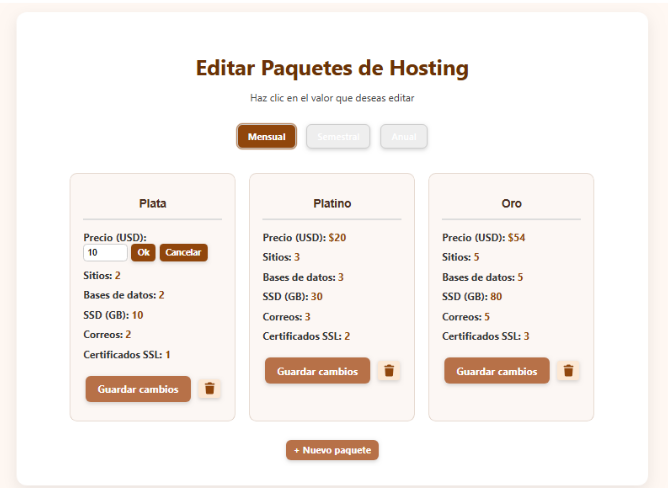
\includegraphics[width=0.7\linewidth]{guiamodulo/gestion-hosting.png}
        \caption{Gestión hosting.}
        \label{fig:gestion-hosting.png}
    \end{figure}

    \item Luego de modificar los valores deseados deber seleccionar “Guardar cambios” en el paquete deseado

    \begin{figure}[H]
        \centering
        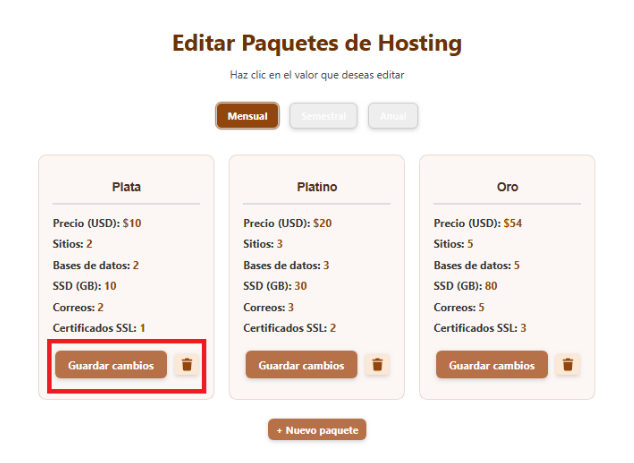
\includegraphics[width=0.7\linewidth]{guiamodulo/gestion-hosting-guardar.png}
        \caption{Gestión hosting, guardar.}
        \label{fig:gestion-hosting-guardar.png}
    \end{figure}

    \item Si todo sale bien, verá el mensaje siguiente

    \begin{figure}[H]
        \centering
        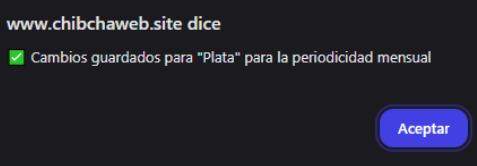
\includegraphics[width=0.4\linewidth]{guiamodulo/gestion-hosting-aviso.png}
        \caption{Gestión hosting, notificación.}
        \label{fig:gestion-hosting-aviso.png}
    \end{figure}

\end{enumerate}

\subsubsection*{Añadir un nuevo paquete de Hosting}
\begin{enumerate}
	\item Desde la vista de Paquete, debe seleccionar la periodicidad e ingresar a “Nuevo Paquete”
	\begin{figure}[H]
        \centering
        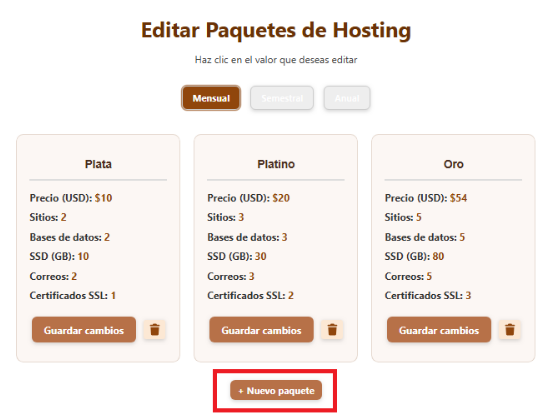
\includegraphics[width=0.7\linewidth]{guiamodulo/gestion-hosting-nuevo.png}
        \caption{Gestión hosting, nuevo paquete.}
        \label{fig:gestion-hosting-nuevo.png}
    \end{figure}

	\item Llene los campos solicitados
	\begin{figure}[H]
        \centering
        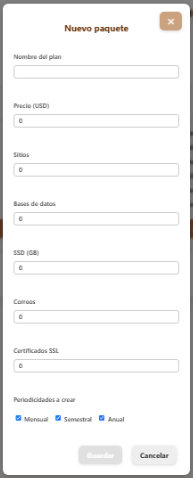
\includegraphics[width=0.2\linewidth]{guiamodulo/gestion-hosting-nuevo-campos.png}
        \caption{Gestión hosting, campos nuevo paquete.}
        \label{fig:gestion-hosting-nuevo-campos.png}
    \end{figure}

    \item De clic en Guardar
\end{enumerate}


\subsubsection {Gestionar perfil }

\begin{enumerate}
\item Para realizar esta acción, se debe dar clic en “Mi perfil”
\begin{figure}[H]
    \centering
    
\includegraphics[width=0.3\linewidth]{guiamodulo/menu-admin-hosting.png}
    \caption{Menú Admin, perfil.}
    \label{fig:menu-admin-perfil}
\end{figure}
\end{enumerate}


\section{Recomendaciones y buenas prácticas}
\subsection{Seguridad de la cuenta}
Con el fin de garantizar la estabilidad, seguridad y eficiencia del sistema ChibchaWeb, se recomienda seguir las siguientes buenas prácticas:

\begin{itemize}
\item Contraseñas seguras: Las contraseñas deben tener al menos 8 caracteres, incluir letras mayúsculas, minúsculas, números y símbolos. Se recomienda usar gestores de contraseñas.

\item Autenticación por rol: Asegúrese de que cada cuenta tenga asignado el tipo de cuenta correcto (Cliente, Distribuidor )
\end{itemize}

\subsection{Uso responsable de recursos}
Todos los usuarios deben utilizar los recursos asignados de manera eficiente y ética. Esto incluye evitar prácticas que puedan afectar el rendimiento del sistema, como el uso excesivo o malintencionado de almacenamiento, ancho de banda o procesamiento. El incumplimiento de estas directrices puede resultar en restricciones temporales o permanentes del servicio.

\subsection{Soporte proactivo}
El sistema cuenta con un módulo de tickets de soporte que permite a los usuarios reportar problemas, realizar consultas y recibir asistencia técnica. El soporte se gestiona de manera proactiva mediante respuestas automáticas inteligentes y seguimiento por parte del equipo de atención, garantizando tiempos de respuesta ágiles y soluciones eficaces para mantener la continuidad del servicio.


\newpage
\section{Glosario}
\subsubsection*{A}

\subsubsection*{B}

\subsubsection*{C}
\begin{itemize}
\item \textbf{Carrito de compra:} Funcionalidad que permite a los usuarios seleccionar, almacenar y gestionar productos o servicios antes de completar una compra.

\item \textbf{Cliente (cuenta):} Usuario registrado en el sistema que adquiere y gestiona servicios como dominios y hosting.

\item \textbf{Comisión:} Porcentaje o monto fijo asignado a distribuidores por ventas realizadas dentro del sistema.

\item \textbf{Cuenta (CUENTA):} Registro individual de usuario dentro del sistema, ya sea cliente, distribuidor, empleado o administrador.
\end{itemize}

\subsubsection*{D}
\begin{itemize}
    \item \textbf{Distribuidor:} Usuario con permisos especiales para revender servicios de dominio/hosting, gestionando clientes y comisiones.
    \item \textbf{Dominio (DOMINIO):} Nombre único que identifica un sitio en Internet, adquirido y gestionado por usuarios dentro del sistema.
\end{itemize}

\subsubsection*{E}
\begin{itemize}
    \item \textbf{Estado del carrito:} Condición actual del carrito de un usuario (abierto, confirmado, pagado, cancelado, etc.).
    \item \textbf{Estado del ticket:} Seguimiento del progreso de un ticket de soporte (pendiente, en proceso, resuelto, cerrado).

\end{itemize}

\subsubsection*{F}

\subsubsection*{G}
\begin{itemize}
    \item \textbf{Gestión de tickets:} Funcionalidad que permite registrar, asignar y resolver solicitudes o incidencias de usuarios.
    \item \textbf{Gestión de dominios:} Módulo que permite registrar, transferir o administrar dominios vinculados a los clientes.
    \item \textbf{Gestión de cuentas:} Funcionalidad administrativa para crear, editar, suspender o eliminar cuentas del sistema.
\end{itemize}

\subsubsection*{H}
\begin{itemize}
\item \textbf {Hosting:} Servicio de alojamiento web que permite publicar sitios y aplicaciones en Internet, con diferentes planes disponibles.
\end{itemize}

\subsubsection*{I}
\begin{itemize}
    \item \textbf {Identificación de cuenta:} Proceso que permite determinar el tipo, estado y permisos de una cuenta específica.
\end{itemize}

\subsubsection*{J}

\subsubsection*{K}

\subsubsection*{L}

\subsubsection*{M}
\begin{itemize}
    \item \textbf {Método de pago:} Forma en que un cliente puede abonar por servicios (tarjeta, transferencia, etc.).
\end{itemize}

\subsubsection*{N}

\subsubsection*{O}

\subsubsection*{P}
\begin{itemize}
    \item \textbf{Paquete de hosting:} Conjunto de servicios agrupados bajo un plan que incluye almacenamiento, ancho de banda, correos, etc.
    \item \textbf{Plan (de hosting):} Nivel de servicio contratado, con características técnicas y precio definido.
\end{itemize}

\subsubsection*{Q}

\subsubsection*{R}
\begin{itemize}
    \item \textbf{Registro de cuenta:} Proceso por el cual un nuevo usuario se da de alta en el sistema.
    \item \textbf{Roles de usuario:} Clasificación de cuentas según sus privilegios (cliente, distribuidor, etc.).
\end{itemize}

\subsubsection*{S}
\begin{itemize}
    \item \textbf{Soporte técnico:} Área dedicada a resolver consultas, problemas o solicitudes de los usuarios del sistema.
    \item \textbf{Sistema de autenticación:} Mecanismo que valida la identidad de usuarios y otorga acceso según sus permisos.
\end{itemize}

\subsubsection*{T}
\begin{itemize}
\item \textbf{Tarjeta (de pago):} Medio electrónico utilizado por los clientes para abonar productos o servicios.
\item \textbf{Ticket:} Solicitud registrada por un cliente relacionada con soporte técnico, facturación, etc.
\item \textbf{Transferencia de dominio:} Proceso mediante el cual un dominio cambia de registrador o de cuenta dentro del sistema.
\item \textbf{Tipo de cuenta:} Clasificación de una cuenta según su función: cliente, distribuidor, etc.
\item \textbf{Tipo de método de pago:} Categoría asignada al método usado para abonar: tarjeta, efectivo, transferencia.
\end{itemize}

\subsubsection*{U}
\begin{itemize}
\item \textbf{Usuario final:} Persona que utiliza el sistema para contratar servicios y administrar su cuenta.
\end{itemize}

\subsubsection*{V}

\subsubsection*{W}

\subsubsection*{X}

\subsubsection*{Y}

\subsubsection*{Z}


\bibliographystyle{plain}
\bibliography{bibliografia/bibliografia}

\end{document}
